% =============================================================================
% File:  sample_slides.tex --  Example of the use of the Falkor Beamer theme
% Author(s): Sebastien Varrette <Sebastien.Varrette@uni.lu>
% Time-stamp: <Mar 2014-04-29 16:06 svarrette>
% 
% Copyright (c) 2012 Sebastien Varrette <Sebastien.Varrette@uni.lu>
% .             http://varrette.gforge.uni.lu
% 
% For more information:
% - LaTeX: http://www.latex-project.org/
% - Beamer: https://bitbucket.org/rivanvx/beamer/
% - LaTeX symbol list:
% http://www.ctan.org/tex-archive/info/symbols/comprehensive/symbols-a4.pdf
% 
% Latest version of these files can be found on Github:
% 

% =============================================================================
\documentclass{beamer}
% \documentclass[draft]{beamer}
\usepackage{_style}
\usepackage{__config}

% The key part to use my theme
\usetheme{Falkor}

% Not integrated in my theme as not everybody wants that
\AtBeginSection[]
{
  \frame{
    \frametitle{Summary}
    {\scriptsize\tableofcontents[currentsection]}
  }
}

%%%%%%%%%%%%%%%%%%%%%%%%%%%% Header %%%%%%%%%%%%%%%%%%%%%%%%%%%%%%
\title{\EventName}
\subtitle{\TPindex: \TPtitle}

\author{\authors}
\institute[UL]{
  University of Luxembourg, Luxembourg
}

% Mandatory to define a logo - otherwise compilation will fail in an unobvious
% manner.
\pgfdeclareimage[height=0.8cm]{logo}{images/logo_UL.pdf}
\logo{\pgfuseimage{logo}}
\date{}

%%%%%%%%%%%%%%%%%%%%%%%%%%%%%% Body %%%%%%%%%%%%%%%%%%%%%%%%%%%%%%%
\begin{document}

\begin{frame}
    \vspace{2.5em}
    \titlepage
\end{frame}

% .......
\frame{
  \begin{center}
      \textbf{Latest versions available on
        \href{https://github.com/ULHPC/}{Github}}:
      \vfill
      \begin{description}
        \item[UL HPC tutorials:] \hfill
          \myurl{https://github.com/ULHPC/tutorials}
        \item[UL HPC School:] \hfill
          \myurl{http://hpc.uni.lu/hpc-school/}
        \item[\TPindex  tutorial sources:] \hfill
          \myurl{\TPghurl}
      \end{description}
  \end{center}
}

% ......
\frame{
  \frametitle{Summary}
  {\scriptsize
    \tableofcontents
  }
}

% ===============================================
\section{Pre-requisites}

% .......
\begin{frame}[fragile]
    \frametitle{Install and Run R}
    \begin{enumerate}
      \item On your local machine:
		\begin{itemize}
			\item Find a release that fits your distribution\\ at CRAN Archive\hfill\myurl{http://cran.r-project.org/}
			\item Install and launch R-Studio\hfill\myurl{https://www.rstudio.com/}
		\end{itemize}
      \item On the cluster\\
       First connect to the cluster, then submit a job to run R.
        \begin{cmdline}
            \cmdlinelocal{ssh chaos-cluster}\\
            \cmdlinefrontend{oarsub -I -l core=1,walltime="00:30:00"}\\
            \cmdlinenode{module load R/3.0.2-ictce-5.3.0}\\
            \cmdlinenode{R}
        \end{cmdline}
        \item Install and Load a Package
            \begin{cmdline}
              \cmdlineR{install.packages("ggplot2")}\\
              \cmdlineR{library(ggplot2)}\\
            \end{cmdline}
    \end{enumerate}
\end{frame}

% ===============================================
\section{Objectives}

% ............
\frame{

  \frametitle{Objectives of this Practical Session}

  \begin{itemize}
    \item Being able to plot data
     \begin{itemize}
      \item histogram for data distribution
      \item plot in different colors from different data sources
     \end{itemize}
    \item Know some tips to organize your data
     \begin{itemize}
      \item aggregate a dataset by column and apply an aggregation function
      \item data.table package for binary search in datasets
      \item performance in R operations
     \end{itemize}     
    \item R in parallel
     \begin{itemize}
      \item on one machine
      \item on a cluster with socket communications
     \end{itemize}
     
\end{itemize}      




}


\section{Practical Session}

% .......
\frame{
  \frametitle{Exercises}
    \begin{itemize}
      \item Start the tutorial \myurl{\TPghurl}
      \begin{itemize} 
	      \item Plot 2 graphs in section Simple Plotting
	      \item Answer 2 questions at the end of section Organizing your Data
	      \item Compare performance of aggregation operations w/wo parallelization
      \end{itemize}
      \item Plot a speedup graph
      \begin{itemize}
       \item with different number of cores and/or machines
       \item needs: ggplot, parallel R
      \end{itemize}
    \end{itemize}
}

\frame{
  \frametitle{Simple Plotting}
  Movies Histogram:
    \begin{center}
       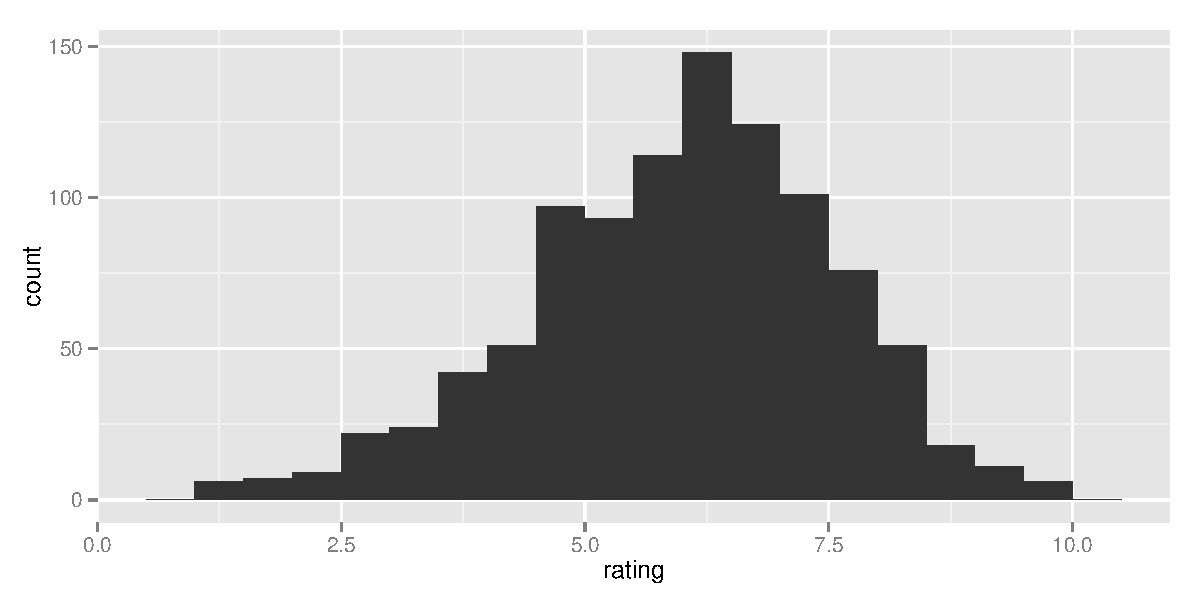
\includegraphics[scale=0.25]{figures/movies_hist.pdf}
    \end{center}
    
    Diamonds Plot with 2 colours:
    \begin{center}
       \hspace{1.8em}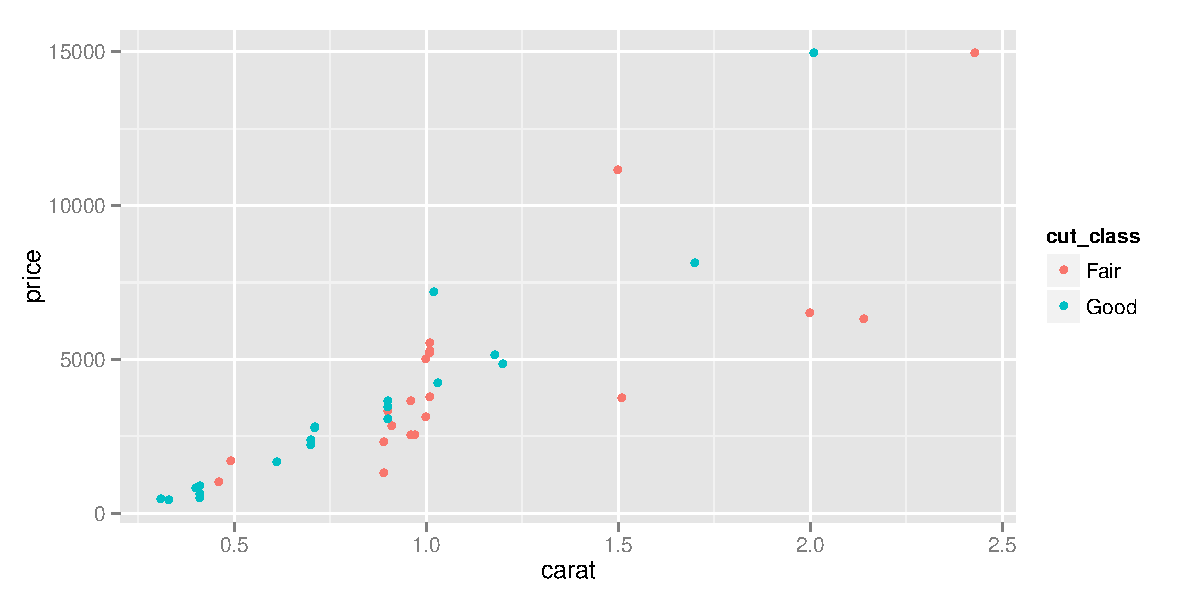
\includegraphics[scale=0.3]{figures/diamonds_plot.pdf}
    \end{center}
}

\frame[containsverbatim]{
  \frametitle{PS Questions}
  \begin{block}{Question: use ddply instead of tapply in the first example}
      \begin{lstlisting}[basicstyle=\tiny,numbers=none]
          ddply(DT, .(x), summarize, sum(v))
      \end{lstlisting}
  \end{block}   
  
  \begin{block}{Question: return the min and max instead of the sum.}
      \begin{lstlisting}[basicstyle=\tiny,numbers=none]
          min_max = function(data){
  			c(min(data), max(data))
		  }
          DT[,min_max(v),by=x]
          
          ## or  
                  
          DT[,c(min(v), max(v)),by=x]	
      \end{lstlisting}
  \end{block}  
}

\section*{Thank you for your attention...}
\frame{
  \frametitle{Questions?}
  \begin{center}
      
\includegraphics[scale=0.2]{question.jpg}
  \end{center}

  {\tiny
    \tableofcontents

  }
}

\newcounter{finalframe}
\setcounter{finalframe}{\value{framenumber}}

% \appendix

\frame{
  \frametitle{Usefull links}

    \begin{itemize}
      \item CRAN Archive \hfill\myurl{http://cran.r-project.org/}
      \item ggplot2 Documentation \hfill\myurl{http://docs.ggplot2.org/current/}
      \item CRAN HPC\\ Packages \hfill\myurl{http://cran.r-project.org/web/views/HighPerformanceComputing.html}
      \item Advanced R programming by Hadley Wickham \hfill\myurl{http://adv-r.had.co.nz/}
    \end{itemize}
}

\setcounter{framenumber}{\value{finalframe}}

\end{document}

% ~~~~~~~~~~~~~~~~~~~~~~~~~~~~~~~~~~~~~~~~~~~~~~~~~~~~~~~~~~~~~~~~
% eof
% 
% Local Variables:
% mode: latex
% mode: flyspell
% mode: auto-fill
% fill-column: 80
% End:
